\section{Diagramas de secuencia}

Los diagramas de secuencia se utilizan para modelar la interacción entre las distintas partes de un sistema según UML. De esta forma, se podrá observar de una forma más ilustrativa el funcionamiento de la aplicación, y las interacciones del usuario con esta última. 
\\

Se han realizado diagramas de secuencia para todas las operaciones realizadas en el sistema, y se pueden observar detenidamente en el \hyperref[enlaceDiagramasSecuencia]{Apéndice D. Diagramas de secuencia}. Para explicar en mayor detalle estos, se explican a continuación los diagramas más importantes y/o representativos de la aplicación.

\section{Página de inicio de sesión}
\label{PInicioSesion}

\begin{figure}[H]
\centerline{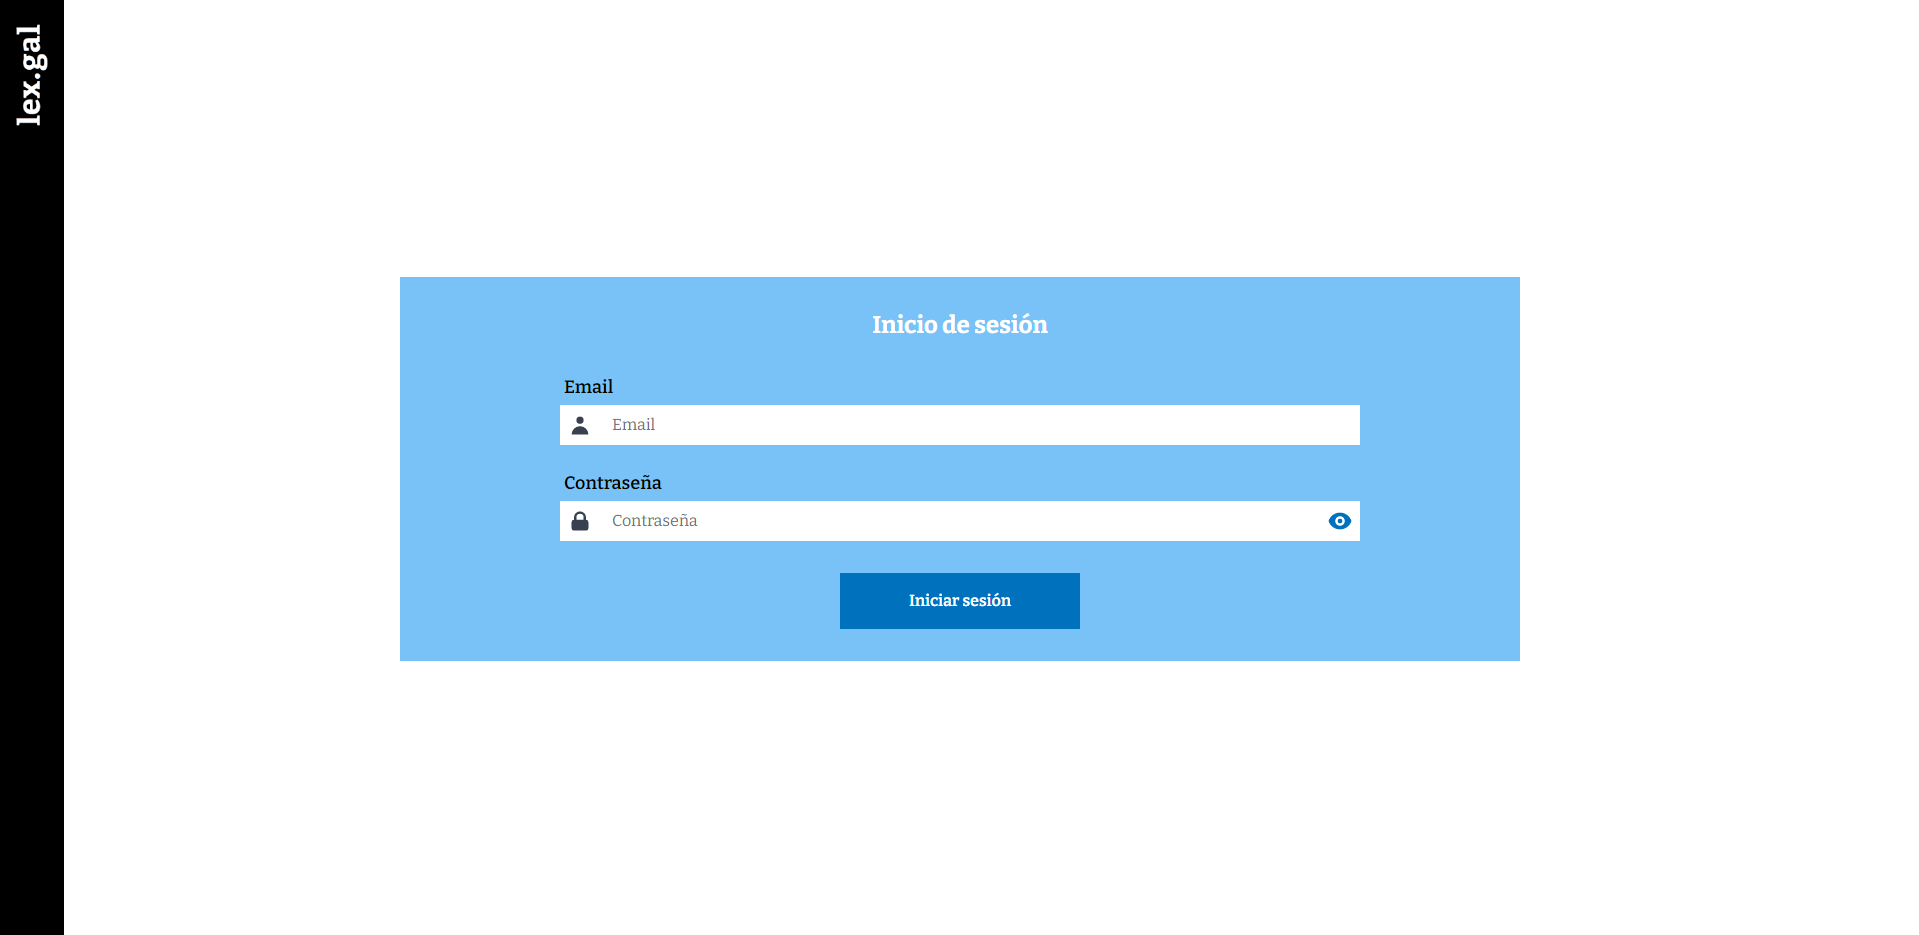
\includegraphics[width=15cm]{figuras/manualUsuario/InicioSesion.PNG}}
\caption{Página de inicio de sesión.}
\label{enlacePInicioSesion}
\end{figure}

En un primer momento el usuario ha de iniciar sesión para poder utilizar la aplicación. En este caso ha de introducir el correo electrónico y su contraseña. Si los datos de inicio de sesión son correctos, será redirigido automáticamente a la página principal de la aplicación. Se puede ver como se ha de hacer en la \hyperref[enlacePInicioSesion]{Figura B.1}.
\subsection{Buscar una ley en lex.gal}

Se representa la operación de búsqueda de leyes en la base de datos de lex.gal. En este caso, puede ser que se encuentren o no leyes, devolviendo las encontradas en el primero de los casos. Esta operación se puede realizar desde las páginas Home y Search del cliente.

\begin{figure}[H]
\centerline{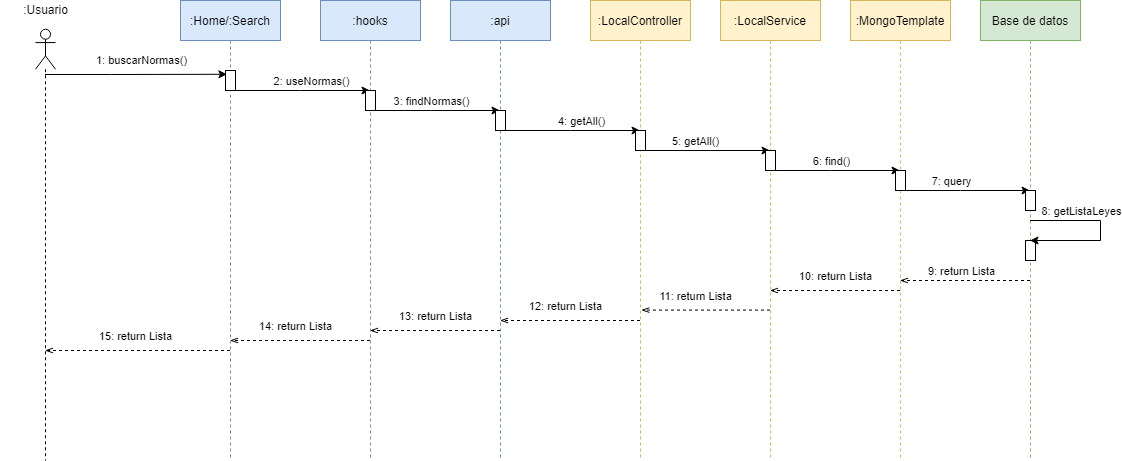
\includegraphics[width=15cm]{figuras/diseño/BuscarLeyLEXGAL.png}}
\caption{Diagrama de secuencia 02. Buscar una ley en lex.gal.}
\label{enlaceDBuscar}
\end{figure}

En la \hyperref[enlaceDRegistro]{Figura 3.9} se ilustra el diagrama de secuencia de la operación de buscar una ley en lex.gal. Se puede resumir en los siguientes pasos:

\begin{enumerate}
    \item El usuario pincha en buscar leyes en la página de búsqueda, con el texto de sumario si este ha escrito algo, o sin él.
    \item Este método invoca al hook useNormas() del archivo contenido en hooks().
    \item Se invoca al método findNormas() de la carpeta {\bf api}.
    \item Se hace un llamamiento mediante una solicitud HTTP al servidor. En concreto, la función getAll() de LocalController, pues se hace un GET.
    \item Se invoca al servicio getAll() de FinalDocumentService.
    \item Se invoca la operación find() del Template MongoTemplate, pues se busca según un texto, páginas y también tamaño de búsqueda.
    \item Se invoca la operación de recuperar en la base de datos de MongoDB.
    \item Se recuperan las leyes encontradas en la base de datos.
    \item Se procede a devolver la respuesta al usuario desde este paso, realizando el proceso inverso. El usuario recibirá las leyes encontradas de forma paginada, según el texto de sumario que había escrito.
\end{enumerate}
\subsection{Editar una ley de lex.gal}

La principal funcionalidad de esta aplicación es la de editar una ley de lex.gal. En esta, un usuario estará visualizando una ley de lex.gal, y procederá a editar sus datos, así como la de las leyes vinculadas. Una vez se ha realizado la edición, el usuario ha de guardar sus cambios, y estos han de ser almacenados en la base de datos.

\begin{figure}[H]
\centerline{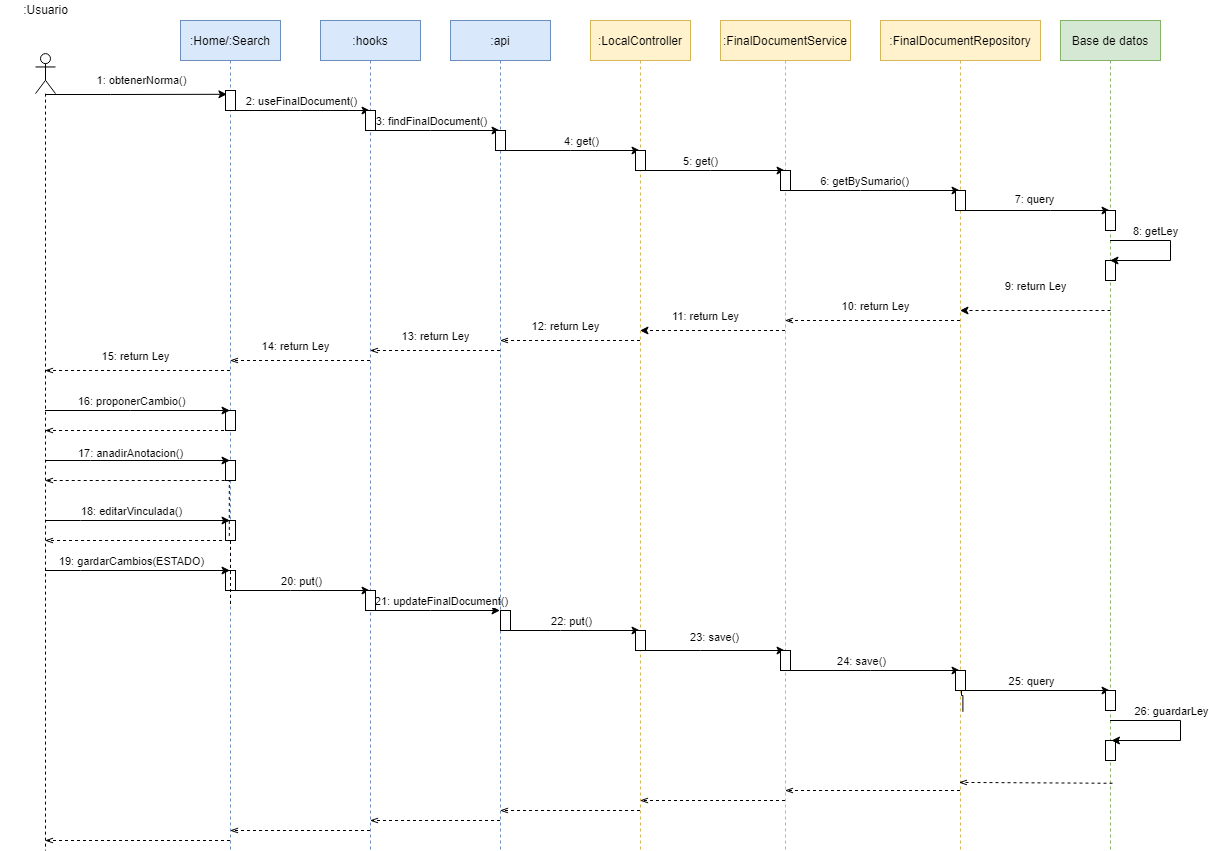
\includegraphics[width=14cm]{figuras/diseño/EditarLey.png}}
\caption{Diagrama de secuencia 03. Editar una ley de lex.gal.}
\label{enlaceDEditar}
\end{figure}

\begin{enumerate}
    \item El usuario pincha entra en la página de edición de una ley, la cual se debe de buscar el método que invoca al hook.
    \item Este método invoca al hook useFinalDocument() del archivo contenido en hooks().
    \item Se invoca al método findFinalDocument() de la carpeta api.
    \item Se hace un llamamiento mediante una solicitud HTTP al servidor. En concreto, la función get() de LocalController, pues se hace un GET.
    \item Se invoca al servicio get() de FinalDocumentService.
    \item Se invoca la operación getBySumario() del repositorio FinalDocumentRepository, pues se busca según el sumario.
    \item Se invoca la operación de recuperar en la base de datos de MongoDB.
    \item Se recupera la leyes encontrada en la base de datos.
    \item Se procede a devolver la respuesta al usuario desde este paso, realizando el proceso inverso. El usuario recibirá las ley correspondiente. Se realiza este proceso {\bf hasta la operación 15}.
    \item El usuario propone cambios que se almacenan en el store de React.
    \item El usuario añade anotaciones que se almacenan en el store de React.
    \item El usuario propone cambios en leyes vinculadas que se almacenan en el store de React.
    \item El usuario guarda los cambios. En función de si valida y publica, o guarda como borrador, tendrá un estado u otro.
    \item Este método invoca al método put() del hook useFinalDocument().
    \item Se invoca al método updateFinalDocument() de la carpeta api.
    \item Se hace un llamamiento mediante una solicitud HTTP al servidor. En concreto, la función put() de LocalController, pues se hace un PUT.
    \item Se invoca al servicio save() de FinalDocumentService.
    \item Se invoca la operación save() del repositorio FinalDocumentRepository, para poder modificar una ley.
    \item Se invoca la operación de modificación en la base de datos de MongoDB.
    \item Se modifica la ley correspondiente en la base de datos.
    \item Se procede a devolver la respuesta al usuario desde este paso, realizando el proceso inverso. El usuario recibirá un mensaje de que la operación fue satisfactoria.
\end{enumerate}